\section{任务一}
\subsection{任务内容}
实现一个简单的类FAT-16文件系统,具有功能:mkdir,ls,delete,open,read,write,close。

\subsection{任务实现规划}
按照实验指导书的提示,实现的是基于内存的简单文件系统,不需要考虑磁盘操作(定义数组模拟磁盘,不需要考虑磁盘的寻道延迟、旋转延迟和传输延迟),也不需要实现SSD的
over-provisioning和garbage collection等。重点考虑实现FAT、目录结构、文件结构以及相应的文件操作等即可。





\subsubsection{常量定义头文件}
在include目录下的fat.h文件中定义所有用到的常量、结构体如下:
\begin{ccode}{常量与结构体定义}
#include<stdio.h>
#include<string.h>
#include<stdlib.h>
#include<stdbool.h>

// 定义所用的常量
#define DISK_SIZE 2560//磁盘大小
#define BLOCK_SIZE 64 //磁盘块大小
#define BLOCK_NUM  (DISK_SIZE / BLOCK_SIZE)
#define MAX_ENTRY 32
#define MAX_OPENFILE 32
#define MAX_FD 16
#define DIR_NAME_LENGTH 16
// 定义模式
#define MODE_READ 1
#define MODE_WRITE 2
#define MODE_RDWR 3
#define MODE_WAPPEND 4  //写追加
// 全局数组声明
extern char Disk[DISK_SIZE];
extern int FAT[BLOCK_NUM]; // FAT表,个数即为块数。
extern int current_dir;//当前目录索引


typedef struct{
    char name[DIR_NAME_LENGTH]; // 目录长度
    int size;
    size_t start_block;
    int ac;//是否使用,0表示未使用,1表示已使用
    int type;//0表示文件,1表示目录
    int parent;
}DirEntry;

typedef struct{
    int used;//0空闲,1已经使用
    int dir_index;//文件下标
    int offset;//读写偏移
    int mode;//打开模式
}FileDescriptor;

extern DirEntry Directory[MAX_ENTRY];
extern FileDescriptor FDTable[MAX_FD]; 
\end{ccode}
上述代码中定义了磁盘大小、磁盘块大小、磁盘块数(磁盘大小/磁盘块大小)以及最大目录项数、最大打开文件数、最大文件描述符数和最大文件名长度。
定义了目录项结构体DirEntry,包含属性目录名、目录大小、起始磁盘块号、是否使用、目录类型(0表示文件,1表示目录)和父目录索引。
定义了文件描述符结构体FileDescriptor,包含属性是否使用、文件下标、读写偏移以及打开模式(对应只读r、只写w和读写rw)。还声明了全局变量
磁盘数组Disk用以描述磁盘;FAT数组表示磁盘块的链接和分配关系;current\_dir表示当前目录位置索引;Directory数组表示目录项;FDTable数组表示文件描述符。
\subsection{函数声明}
在include目录下的fat.h中声明了实现该FAT-16文件系统所用到的函数,代码如下:
\begin{ccode}{函数声明}
//初始化
void init_fs(void);
void init_fd_table(void);

//目录
bool fs_mkdir(const char *dirame);
bool fs_ls(void);
bool fs_cd(const char *direname);


//文件创建与删除
bool fs_create(const char *filename);
bool fs_delete(const char *filename);

//文件操作,读写
int fs_open(const char * filename,int mode); //返回文件描述符fd
bool fs_close(int fd);
int fs_write(int fd,const char *data,int size);
int fs_read(int fd,char *buffer,int size);
bool fs_seek(int fd,int offset);


//打印提示
void print_prompt(void);

bool cd(const char *filename);
bool ls();
bool mkdir(const char *dirname);
\end{ccode}
其中主要包括了系统初始化函数、目录操作函数、文件操作函数(目录的创建、删除和切换当前位置,文件的创建、删除、打开、关闭、读写和定位)以及辅助打印信息函数。
\subsubsection{文件系统初始化}
在src文件夹中的init.c文件中实现对该文件系统的初始化,代码如下:
\begin{ccode}{文件系统初始化}
#include "fat.h"
#include<string.h>

// 全局变量定义
char Disk[DISK_SIZE];
int FAT[BLOCK_NUM];
int current_dir;
DirEntry Directory[MAX_ENTRY];
FileDescriptor FDTable[MAX_FD];

void init_fd_table(void){
    memset(FDTable,0,sizeof(FDTable));
    for (int i = 0; i < MAX_FD;i++){
        FDTable[i].dir_index = -1;
    }
}

void init_fs(void){
    memset(Disk,0,sizeof(Disk));
    memset(FAT,0,sizeof(FAT));
    memset(Directory,0,sizeof(Directory));
    for (int i = 0;i < MAX_ENTRY; i++){
        Directory[i].start_block = -1;
        Directory[i].parent = -1;
    }
    strcpy(Directory[0].name,"/");
    Directory[0].size = 0;
    Directory[0].start_block = -1;
    Directory[0].ac = 1;
    Directory[0].type = 1;
    Directory[0].parent = -1;
    current_dir = 0;
    init_fd_table();
}
\end{ccode}
其中包括对磁盘数组、FAT表、目录项数组和文件描述符数组的全部清零和对根目录的特殊初始化(确认已分配,类型为目录,父目录索引为-1),表示当前位置的全局变量current\_dir置为0,确保初始化后当前处于根目录。


% 目录操作函数
\subsubsection{文件目录操作函数}
在src文件夹中的dir.c文件中实现对目录的相关操作,包括创建文件夹、列出当前目录下所有文件及文件夹、切换目录等。具体代码如下:
\begin{ccode}{目录操作函数}
#include "fat.h"

//mkdir

bool mkdir(const char *dirname){
    for (int i = 0; i < MAX_ENTRY;i++){
        if (Directory[i].ac == 0)//找到空闲目录项
        {
            strncpy(Directory[i].name,dirname,DIR_NAME_LENGTH);
            Directory[i].size = 0;
            Directory[i].start_block = -1;
            Directory[i].ac = 1;
            Directory[i].type = 1;//1表示目录
            Directory[i].parent = current_dir;//设置父目录索引
            return true;
        }
    }
    return false; // 目录创建失败返回false
}

int get_dir_size(int dir_index){
    int total = 0;
    
    for (int i = 0; i < MAX_ENTRY; i++){
        if (Directory[i].ac == 1 && Directory[i].parent == dir_index){
            if (Directory[i].type == 0){
                //普通文件
                total += Directory[i].size;            
            }else if (Directory[i].type == 1){
                //目录文件,递归统计
                total += get_dir_size(i);
            }
        }
    }
    return total;//统计dir_index号目录下的文件、目录项总个数
}

//ls
bool ls(){
    for (int i = 0; i < MAX_ENTRY;i++){
        //遍历所有Directory,已分配且在当前目录下的文件和目录list出来
        if (Directory[i].ac == 1 && Directory[i].parent == current_dir){
            int show_size;
            if (Directory[i].type == 1){
                show_size = get_dir_size(i);
            }else{
                show_size = Directory[i].size;
            }

            printf("%s\t%s\t%d bytes\n",
            Directory[i].type == 1 ? "DIR":"FILE",
            Directory[i].name,
            show_size
            );
        }
    }
    return true;
}

// cd 
bool cd(const char *dirname){
    if (dirname == NULL) return false;

    // 回到根目录
    if (strcmp(dirname,"/") == 0){
        current_dir = 0;
        return true;
    }
    
    // 回到父目录
    if (strcmp(dirname,"..") == 0){
        if(Directory[current_dir].parent != -1){//根目录往上翻还是在根目录
            current_dir = Directory[current_dir].parent;
        }
        return true;
    }
    

    //进入下级目录
    for (int i = 0; i < MAX_ENTRY; i++){
        if (Directory[i].ac == 1 && Directory[i].parent == current_dir && Directory[i].type == 1 && 
            strcmp(Directory[i].name,dirname) == 0){
                current_dir = i;
                return true;
            }
    }
    return false;
}
\end{ccode}
其中新建文件夹就是在Directory数组中找一个空闲目录项,将其设置为指定的新建目录项并更新对应的父目录索引、大小、类型等。
辅助函数get\_dir\_size()采用递归的方式,统计指定目录下所有文件及子目录的总大小。ls()函数用于列出当前目录下所有文件及文件夹,打印出对应的类型、文件名和大小,实现
方法为遍历Directory数组,已分配且父目录索引等于当前目录项索引的即为当前目录下的文件、文件夹。cd()函数用于切换当前目录,事实上只需要改变存放当前目录位置的全局变量
即可实现切换。为了简化,只实现了切换到根目录('/')、父目录('..')和切换到下级指定文件夹的功能。另外为了鲁棒性,当处于根目录时,切换到根目录操作会被跳过,不会重复改变当前目录。

\subsubsection{文件的打开与关闭}
在src文件夹中的fd.c文件中实现对文件的打开与关闭,这里打开与关闭文件是便于后续对文件的读写操作,具体代码如下:
\begin{ccode}{文件的打开与关闭}
#include "fat.h"

int fs_open(const char *filename,int mode){
    if (filename == NULL) return -1;

    //在当前目录下找普通文件
    int  dir_idx = -1;
    for(int i = 0; i < MAX_ENTRY; i++){
        if(Directory[i].ac == 1 &&
            Directory[i].parent == current_dir &&
            Directory[i].type == 0&&
            strcmp(Directory[i].name,filename) == 0
        ){
            dir_idx = i;
            break;
        }
    }
    if (dir_idx == -1){
        //没有找到
        printf("open failed : file not found : %s \n",filename);
        return -1;
    }

    // 找空闲fd
    for (int fd = 0; fd < MAX_FD; fd ++){
        if(FDTable[fd].used == 0){
            FDTable[fd].used = 1;
            FDTable[fd].dir_index = dir_idx;
            FDTable[fd].offset = 0;
            FDTable[fd].mode = mode;
            printf("open success : %s,fd = %d\n",filename,fd);
            return fd;
        }  
    }
    printf("open failed:too many open files\n");
    return -1;
}

bool fs_close(int fd){
    //无效fd
    if (fd < 0 || fd > MAX_FD){
        printf("close failed : invalid fd\n");
        return false;
    }
    //文件还未打开
    if(FDTable[fd].used == 0){
        printf("close failed : fd is not open yet\n");
        return false;
    }
    //正常关闭文件
    FDTable[fd].used = 0;
    FDTable[fd].dir_index = -1;
    FDTable[fd].offset = 0;
    FDTable[fd].mode = 0;
    printf("close success: fd = %d\n", fd);
    return true;
}

bool fs_seek(int fd,int offset){
    if(fd < 0 || fd >= MAX_FD) return false;
    if(FDTable[fd].used == 0) return false;
    if(offset < 0) return false;

    int dir_idx = FDTable[fd].dir_index;
    int file_size = Directory[dir_idx].size;

    // 读模式不允许超过文件大小
    if(FDTable[fd].mode == MODE_READ || FDTable[fd].mode == MODE_RDWR){
        if(offset > file_size){
            printf("seek failed: offset %d exceeds file size %d\n", offset, file_size);
            return false;
        }
    }

    FDTable[fd].offset = offset;
    return true;
}
\end{ccode}
其中fs\_open()函数用于打开当前目录下指定文件名的文件(这里为了简化实现,没有实现打开任意目录下的文件),通过遍历Directory数组,找到不为空、文件名为指定文件且父目录为当前目录的文件即为要打开的文件,找不到就返回失败并打印错误信息。
找到后再在FDTable数组(即打开文件表)中查找未使用的项,将其信息同步为当前要打开的文件,并将FDTable数组中对应项的索引返回(即文件描述符),后续对文件的读写操作都基于该索引。fs\_close()函数用于关闭指定文件,因为确定只有确定已经打开的文件
才需要关闭,因此这里关闭文件函数接收的参数为文件描述符fd。具体实现为检查fd未越界且FDTable数组中对应表项不为空时,将这一项清零即可。
fs\_seek()函数用于设置文件从何处开始读写,通过接收参数文件描述符fd和偏移量offset,在确认都没有越界的情况下更新FDTable中对应项的offset属性即可。

\subsection{文件读写与删除}
在src文件夹中的file.c文件中实现文件的读写与删除功能,具体包括文件的创建、读写和删除操作,具体代码分别如下:
\begin{itemize}
    \item 文件创建函数:
    \begin{ccode}{文件创建}
// 创建文件，写文件
bool fs_create(const char*filename){
    for (int i = 0; i < MAX_ENTRY; i++){
        if(Directory[i].ac == 0){
            // 找到空闲块
            strncpy(Directory[i].name,filename,DIR_NAME_LENGTH);
            Directory[i].size = 0;
            Directory[i].start_block = -1;
            Directory[i].ac = 1; 
            Directory[i].type = 0;//0表示文件
            Directory[i].parent = current_dir; //设置父目录索引
            printf("File created successfully : %s\n",filename);
            return true;
        }
    }
    printf("Failed to created file : %s\n",filename);
    return false;
}
    \end{ccode}
    文件创建就是接收参数文件名filename,在Directory数组中找一个空闲块,并设置该块对应属性,包括文件名、文件大小、文件类型、是否被分配以及父目录索引。
    \item 写文件函数:
    \begin{ccode}{写文件函数}
int fs_write(int fd,const char* data,int size){
    if(fd < 0 || fd >= MAX_FD || data == NULL || size < 0) return -1;
    if(FDTable[fd].used == 0){
        printf("write failed : fd is not open\n");
        return -1;
    }

    if(FDTable[fd].mode != MODE_WRITE && FDTable[fd].mode != MODE_RDWR && FDTable[fd].mode != MODE_WAPPEND){
        printf("write failed : fd is not writable");
        return -1;
    }

    if (size == 0){
        return 0;
    }

    int dir_index = FDTable[fd].dir_index;
    int offset = FDTable[fd].offset;
    int end_pos = offset + size;

    int need_blocks = (end_pos + BLOCK_SIZE - 1) / BLOCK_SIZE;

    // 确保文件有足够多的 block
    if (Directory[dir_index].start_block == -1) {
        int new_block = -1;

        for (int i = 0; i < BLOCK_NUM; i++) {
            if (FAT[i] == 0) {
                new_block = i;
                break;
            }
        }

        if (new_block == -1) {
            printf("write failed: no free block\n");
            return -1;
        }

        FAT[new_block] = -1;
        memset(Disk + new_block * BLOCK_SIZE, 0, BLOCK_SIZE);
        Directory[dir_index].start_block = new_block;
    }

    int cur = Directory[dir_index].start_block;
    int block_count = 1;

    while (FAT[cur] != -1) {
        cur = FAT[cur];
        block_count++;
    }

    while (block_count < need_blocks) {
        int new_block = -1;

        for (int i = 0; i < BLOCK_NUM; i++) {
            if (FAT[i] == 0) {
                new_block = i;
                break;
            }
        }

        if (new_block == -1) {
            printf("write failed: no enough space\n");
            return -1;
        }

        FAT[new_block] = -1;
        memset(Disk + new_block * BLOCK_SIZE, 0, BLOCK_SIZE);

        FAT[cur] = new_block;
        cur = new_block;
        block_count++;
    }

    //找offset对应的block
    int block_index = offset / BLOCK_SIZE;
    int block_offset = offset % BLOCK_SIZE;

    cur = Directory[dir_index].start_block;

    for(int i = 0; i < block_index;i++){
        cur = FAT[cur];
    }

    // 从offset 开始写数据
    int bytes_written = 0;
    while (cur != -1 && bytes_written < size){
        int write_size = BLOCK_SIZE - block_offset;

        if(write_size > size - bytes_written){
            write_size = size - bytes_written;
        }
        memcpy(
            Disk + cur * BLOCK_SIZE + block_offset,
            data + bytes_written,
            write_size
        );
        bytes_written += write_size;
        block_offset = 0;
        if(bytes_written < size){
            cur = FAT[cur];
        }
    }

    //更新offset和文件大小

    FDTable[fd].offset += bytes_written;
    if(FDTable[fd].offset > Directory[dir_index].size){
        Directory[dir_index].size = FDTable[fd].offset;
    }

    return bytes_written;
}
    \end{ccode}
    写文件函数接收参数文件描述符fd,数据指针data以及数据大小size,实际写入前需要确保fd有效且文件可写,同时确保FAT中有足够的多的块写入内容(否则写文件失败),最后根据offset确认写入的块的位置并写入data。
    \item 读文件函数:
    \begin{ccode}{读文件函数}
int fs_read(int fd,char *buffer,int size){

    if (fd < 0 || fd >= MAX_FD || buffer == NULL || size < 0) {
        return -1;
    }

    if (FDTable[fd].used == 0) {
        printf("read failed: file is not open\n");
        return -1;
    }

    if (FDTable[fd].mode != MODE_READ && FDTable[fd].mode != MODE_RDWR ){
        printf("read failed : file is not readable\n");
        return -1;
    }
    int dir_index = FDTable[fd].dir_index;
    int file_size = Directory[dir_index].size;
    int offset = FDTable[fd].offset;

    if (offset >= file_size) {
        buffer[0] = '\0';
        return 0;
    }

    int bytes_to_read = size;
    if (offset + bytes_to_read > file_size) {
        bytes_to_read = file_size - offset;
    }

    int bytes_read = 0;
    int cur = Directory[dir_index].start_block;
    int skip_blocks = offset / BLOCK_SIZE;
    int block_offset = offset % BLOCK_SIZE;

    // 跳到 offset 所在的块
    for (int i = 0; i < skip_blocks && cur != -1; i++) {
        cur = FAT[cur];
    }

    while (cur != -1 && bytes_read < bytes_to_read) {
        int read_size = BLOCK_SIZE - block_offset;

        if (read_size > bytes_to_read - bytes_read) {
            read_size = bytes_to_read - bytes_read;
        }

        memcpy(
            buffer + bytes_read,
            Disk + cur * BLOCK_SIZE + block_offset,
            read_size
        );

        bytes_read += read_size;
        block_offset = 0;
        cur = FAT[cur];
    }

    buffer[bytes_read] = '\0';
    FDTable[fd].offset += bytes_read;

    return bytes_read;
}
    \end{ccode}
    读文件函数接收参数文件描述符fd,数据指针buffer以及要读的数据大小size,类似写文件函数,同样要确保fd有效且文件可读,同时根据offset确认读取的块的位置并读取数据。
    \item 删除文件函数:
    \begin{ccode}{删除文件函数}
bool fs_delete(const char *filename){
    for (int i = 0 ; i < MAX_ENTRY; i ++){
        if(Directory[i].ac == 1 && Directory[i].parent == current_dir && Directory[i].type == 0 && strcmp(Directory[i].name,filename) == 0){
            //文件占用的磁盘块在FAT中全部标记为0
            int cur = Directory[i].start_block;
            while (cur != -1){
                int next = FAT[cur];
                FAT[cur] = 0;
                if(next == -1){//找到末尾块
                    break;
                }
                cur = next;
            }
            Directory[i].ac = 0;
            printf("File deleted successfully : %s \n",filename);
            return true;
        }
    }

    printf("Failed to delete file: %s\n", filename);
    return false;
}
    \end{ccode}
    删除文件函数类似文件创建函数,接收参数文件民名filename,然后在Directory数组中查找该文件,找到后释放该文件占用的所有FAT块(从start\_block开始全部置0),并设置为未分配状态即可。
   \end{itemize}

\subsubsection{文件系统入口}
在src文件夹中的main函数中实现整个文件系统的入口,实现思路为先初始化文件系统,然后在死循环中等待用户输入命令,利用之前实现的基础的文件和目录操作函数来实现复杂用户命令,具体代码如下:
\begin{ccode}
#include "fat.h"

void print_path_recursive(int dir){
    if(dir == 0){
        printf("/");
        return;
    }

    int parent = Directory[dir].parent;
    print_path_recursive(parent);

    if (parent != 0){
        printf("/");
    }

    printf("%s",Directory[dir].name);
}

void print_prompt(){
    printf("SimpleFAT:");
    print_path_recursive(current_dir);
    printf("$ ");
}

int main(){
    char line[256];
    char cmd[32];
    char arg1[64];
    char arg2[128];
    char buffer[1024];

    init_fs();

    while(1){
        print_prompt();
        if(fgets(line,sizeof(line),stdin) == NULL){
            break;
        }
        //fgets会读入\n
        line[strcspn(line,"\n")] = '\0';
        if (strlen(line) == 0){
            continue;
        }
        cmd[0] = '\0';
        arg1[0] = '\0';
        arg2[0] = '\0';

        sscanf(line, "%31s %63s %127[^\n]", cmd, arg1, arg2);
        if (strcmp(cmd, "exit") == 0) {
            break;
        }

        else if (strcmp(cmd, "ls") == 0) {
            ls();
        }

        else if (strcmp(cmd, "mkdir") == 0) {
            if (strlen(arg1) == 0) {
                printf("usage: mkdir dirname\n");
            } else if (!mkdir(arg1)) {
                printf("mkdir failed: %s\n", arg1);
            }
        }

        else if (strcmp(cmd, "cd") == 0) {
            if (strlen(arg1) == 0) {
                printf("usage: cd dirname\n");
            } else if (!cd(arg1)) {
                printf("cd failed: %s\n", arg1);
            }
        }

        else if (strcmp(cmd, "touch") == 0) {
            if (strlen(arg1) == 0) {
                printf("usage: touch filename\n");
            } else {
                fs_create(arg1);
            }
        }

        else if (strcmp(cmd, "rm") == 0) {
            if (strlen(arg1) == 0) {
                printf("usage: rm filename\n");
            } else {
                fs_delete(arg1);
            }
        }

        else if (strcmp(cmd, "open") == 0) {
            if (strlen(arg1) == 0 || strlen(arg2) == 0) {
                printf("usage: open filename mode\n");
                printf("mode: r | w | rw\n");
                continue;
            }

            int mode;

            if (strcmp(arg2, "r") == 0) {
                mode = MODE_READ;
            } else if (strcmp(arg2, "w") == 0) {
                mode = MODE_WRITE;
            } else if (strcmp(arg2, "rw") == 0) {
                mode = MODE_RDWR;
            } else {
                printf("invalid mode: %s\n", arg2);
                continue;
            }

            int fd = fs_open(arg1, mode);
            if (fd >= 0) {
                printf("opened fd = %d\n", fd);
            }
        }

        else if (strcmp(cmd, "close") == 0) {
            if (strlen(arg1) == 0) {
                printf("usage: close fd\n");
            } else {
                int fd = atoi(arg1);
                fs_close(fd);
            }
        }

        else if (strcmp(cmd, "write") == 0) {
            if (strlen(arg1) == 0 || strlen(arg2) == 0) {
                printf("usage: write fd content\n");
            } else {
                int fd = atoi(arg1);
                fs_write(fd, arg2, strlen(arg2));
            }
        }

        else if (strcmp(cmd, "read") == 0) {
            if (strlen(arg1) == 0) {
                printf("usage: read fd [size]\n");
                printf("  if size omitted, reads entire file from current offset\n");
            } else {
                int fd = atoi(arg1);

                if (fd < 0 || fd >= MAX_FD || FDTable[fd].used == 0) {
                    printf("read failed: invalid fd %d\n", fd);
                    continue;
                }

                int size;
                if (strlen(arg2) == 0) {
                    // 未指定 size，读取文件剩余全部内容
                    int dir_idx = FDTable[fd].dir_index;
                    int file_size = Directory[dir_idx].size;
                    int offset = FDTable[fd].offset;
                    size = file_size - offset;
                    if (size <= 0 || size > (int)sizeof(buffer) - 1) {
                        size = (int)sizeof(buffer) - 1;
                    }
                } else {
                    size = atoi(arg2);
                }

                int n = fs_read(fd, buffer, size);

                if (n >= 0) {
                    buffer[n] = '\0';
                    printf("%s\n", buffer);
                }
            }
        }

        else if (strcmp(cmd, "cat") == 0) {
            if (strlen(arg1) == 0) {
                printf("usage: cat filename\n");
            } else {
                int fd = fs_open(arg1, MODE_READ);
                if (fd >= 0) {
                    char cat_buf[1024];
                    int n = fs_read(fd, cat_buf, sizeof(cat_buf) - 1);
                    if (n >= 0) {
                        cat_buf[n] = '\0';
                        printf("%s\n", cat_buf);
                    }
                    fs_close(fd);
                }
            }
        }

        else if (strcmp(cmd, "seek") == 0) {
            if (strlen(arg1) == 0 || strlen(arg2) == 0) {
                printf("usage: seek fd offset\n");
            } else {
                int fd = atoi(arg1);
                int offset = atoi(arg2);

                if (!fs_seek(fd, offset)) {
                    printf("seek failed\n");
                }
            }
        }

        else if (strcmp(cmd, "cls") == 0) {
            printf("\033[2J\033[H");
            fflush(stdout);
        }

        else if (strcmp(cmd, "help") == 0) {
            printf("commands:\n");
            printf("  ls\n");
            printf("  mkdir dirname\n");
            printf("  cd dirname\n");
            printf("  touch filename\n");
            printf("  rm filename\n");
            printf("  cat filename\n");
            printf("  open filename r|w|rw\n");
            printf("  close fd\n");
            printf("  write fd content\n");
            printf("  read fd [size]\n");
            printf("  seek fd offset\n");
            printf("  cls\n");
            printf("  exit\n");
        }

        else {
            printf("unknown command: %s\n", cmd);
            printf("type 'help' for help\n");
        }
    }
    return 0;
}
\end{ccode}
其中print\_path\_recursive()函数采用递归的方式打印当前路径;print\_prompt()函数用于实现类似打印当前路径提示符;main()函数中
通过接收用户输入命令参数,在if-else分支中根据不同命令参数调用不同函数实现文件系统功能,如cat命令实现读一个文件内容并打印出来,采用的就是open+read+close的组合实现。(这里没有实现Linux中完整的cat命令所有功能,只是实现了查看指定文件名文件功能)。

\subsubsection{FAT-16文件系统使用测试}
将上述实现的FAT-16文件系统编译后运行,测试结果如下:
\begin{figure}[H]
    \centering
    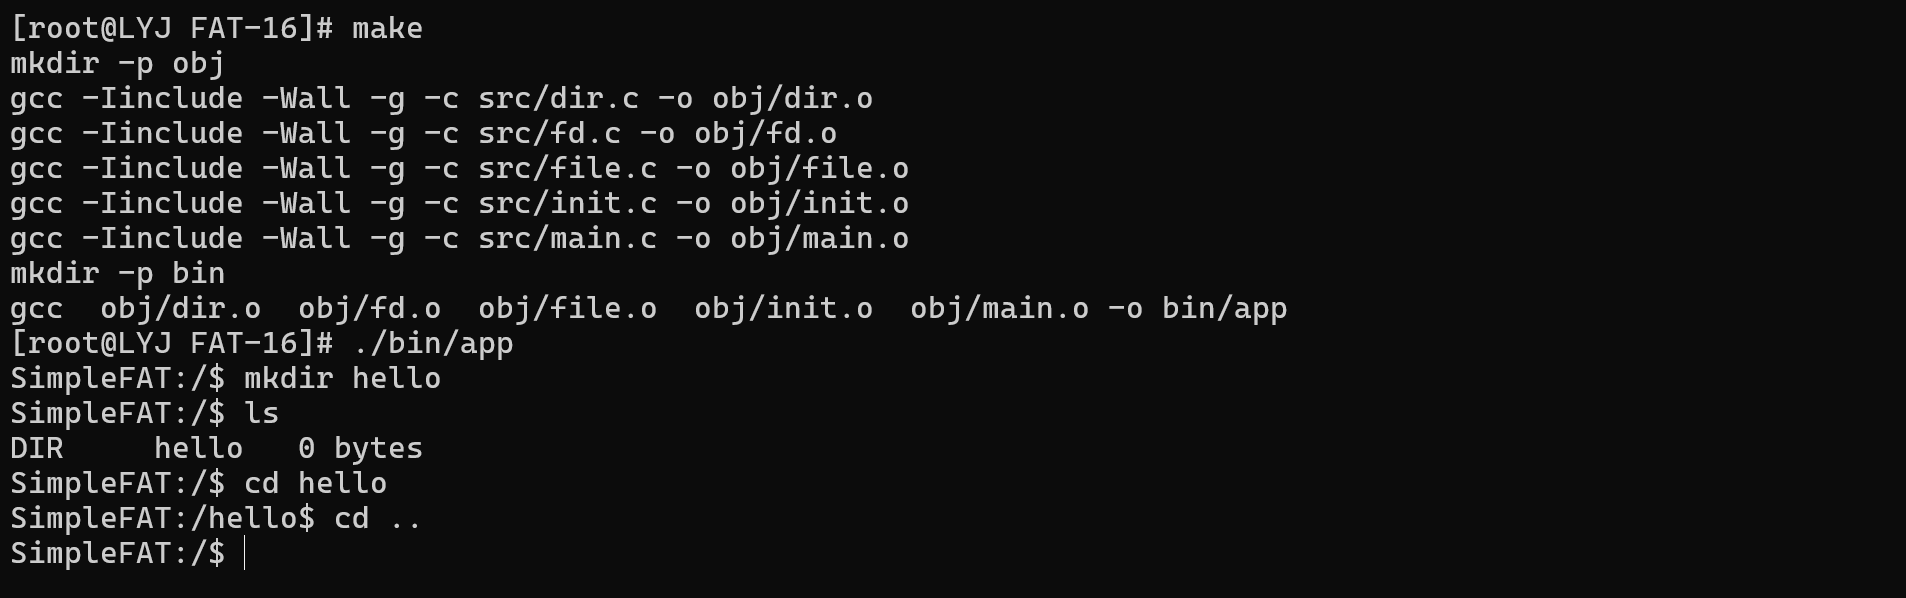
\includegraphics[width = 1\textwidth]{figure/mkdir_cd.png}
    \caption{创建文件夹和切换目录}
\end{figure}
\begin{figure}[H]
    \centering
    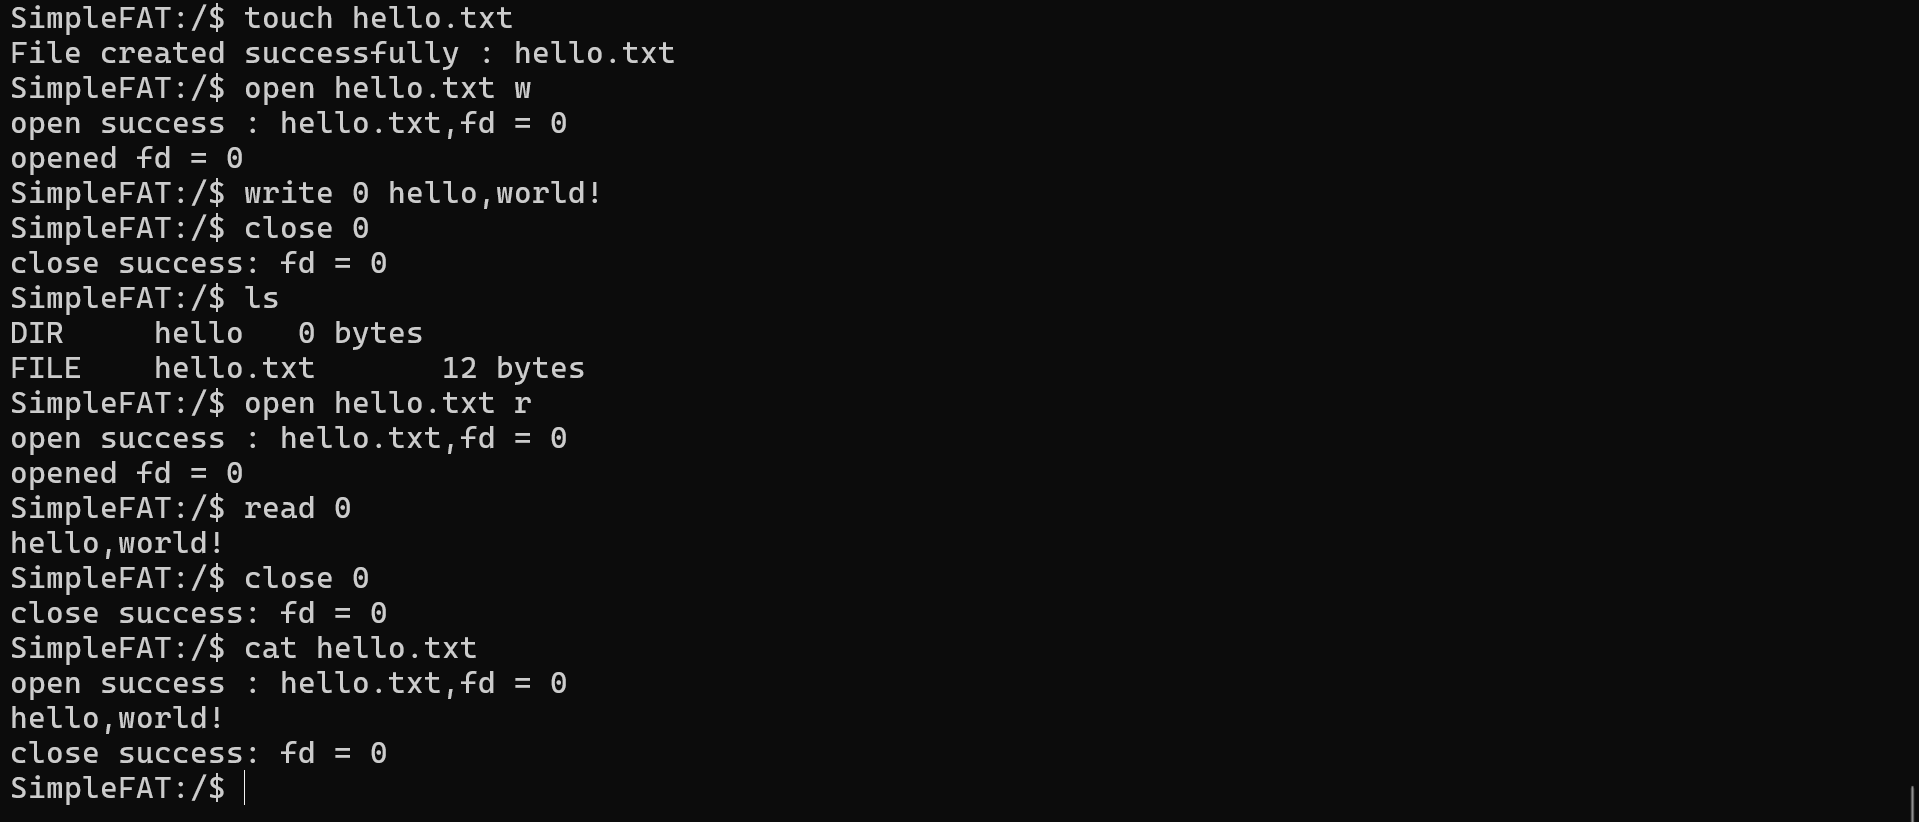
\includegraphics[width = 1\textwidth]{figure/touch_read_write.png}
    \caption{创建文件和读写文件}
\end{figure}

\begin{figure}[H]
    \centering
    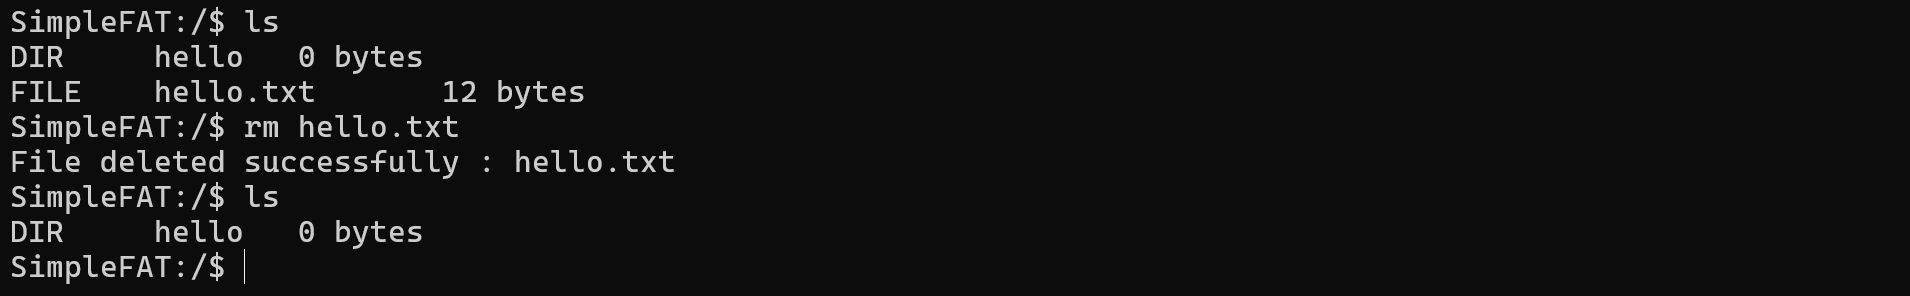
\includegraphics[width = 1\textwidth]{figure/delete.png}
    \caption{删除文件}
\end{figure}
从上述测试结果截图可以看到,该FAT-16文件系统能成功实现基于内存的单进程文件系统,正确完成了mkdir、ls、cd、touch、cat、open、read、write、close、rm等功能,任务一成功完成。

\subsection{任务一函数汇总}
下表对任务一实现的所有主要函数进行汇总,以便对照查阅。

\begin{table}[H]
\centering
\caption{任务一主要函数汇总}
\label{tab:task1_summary}
\resizebox{\textwidth}{!}{%
\begin{tabular}{|c|c|c|c|}
\hline
\textbf{函数名} & \textbf{功能} & \textbf{实现方法} & \textbf{关键数据结构} \\
\hline
\texttt{init\_fs()} & 初始化文件系统 & 清零Disk/FAT/Directory数组,初始化根目录项 & Disk[], FAT[], Directory[] \\
\hline
\texttt{init\_fd\_table()} & 初始化文件描述符表 & memset清零,dir\_index置为-1 & FDTable[] \\
\hline
\texttt{mkdir()} & 创建目录 & 遍历Directory找空闲项,设置目录名/类型/父目录索引 & Directory[] \\
\hline
\texttt{ls()} & 列出当前目录内容 & 遍历Directory,匹配parent==current\_dir,打印类型/名称/大小 & Directory[], current\_dir \\
\hline
\texttt{cd()} & 切换当前目录 & 修改current\_dir,支持/、..、下级子目录名 & Directory[], current\_dir \\
\hline
\texttt{fs\_create()} & 创建文件 & 在Directory中找空闲项,设置文件名/类型/父目录索引 & Directory[] \\
\hline
\texttt{fs\_open()} & 打开文件 & 遍历Directory查找文件→在FDTable中分配空闲表项→返回fd & Directory[], FDTable[] \\
\hline
\texttt{fs\_close()} & 关闭文件 & 验证fd有效性→将FDTable对应表项清零 & FDTable[] \\
\hline
\texttt{fs\_read()} & 读取文件内容 & 从offset所在块开始,沿FAT链逐块memcpy到buffer & Disk[], FAT[], FDTable[] \\
\hline
\texttt{fs\_write()} & 写入文件内容 & 确保FAT链有足够块→从offset逐块写入data→更新文件大小 & Disk[], FAT[], FDTable[] \\
\hline
\texttt{fs\_delete()} & 删除文件 & 沿FAT链释放所有块(FAT标记为0),目录项标记为未使用 & Directory[], FAT[] \\
\hline
\texttt{fs\_seek()} & 设置读写偏移 & 验证fd和offset有效性→更新FDTable中offset字段 & FDTable[] \\
\hline
\end{tabular}%
}
\end{table}

